\documentclass[hyperref=colorlinks]{beamer}
\mode<presentation>
\usetheme{iclpt}
\setbeamertemplate{navigation symbols}{}
\setbeamertemplate{headline}{
\begin{beamercolorbox}[leftskip=.2cm,rightskip=.2cm,topskip=.2cm,ht=1.1cm,dp=0.1cm,wd=\textwidth]{institute in head/foot}
  
\includegraphics[height=1cm]{icl.pdf}
  \hfill
  
\includegraphics[height=1cm]{../Pics/CMS-Color.pdf}
\end{beamercolorbox}
}
\setbeamertemplate{footline}{
\begin{beamercolorbox}[ht=.55cm,dp=0.4cm,wd=\textwidth,leftskip=.3cm]{author in head/foot}%
  \begin{minipage}[c]{5cm}%
    \usebeamerfont{author in head/foot}
    \insertshortauthor 
    \insertshorttitle
    \end{minipage}\hfill%
  \insertframenumber{} / \pageref{lastframe}
  \hfill
  \begin{minipage}{6cm}
    \hfill
  \end{minipage}
\end{beamercolorbox}%
}

\usepackage{color}
\usepackage{tabularx,colortbl}
\usepackage{graphicx}
\usepackage{pdfpages}
\usepackage{feynmp}
\DeclareGraphicsRule{*}{mps}{*}{}

\title{\vspace{-0.2cm} VBF Higgs to Invisible}
\subtitle{HIG-14-038, AN-14-243\vspace{-0.7cm}}
\author[]{}%\underline{P. Dunne}} % A.M. Magnan and A. Nikitenko Joao Pela with \\ R. Aggleton, J. Brooke: Bristol \\ C.Asawangtrakuldee, Q.Li: Peking \\ P. Srimanobhas: Chulalongkorn \\ S. Kumar, K. Mazumdar: Mumbai}
\titlegraphic{
  \vspace{-0.7cm}
  %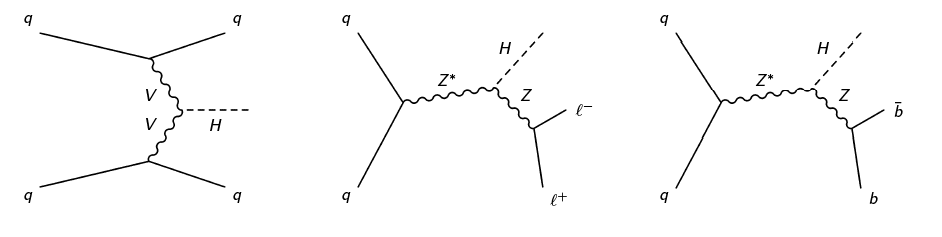
\includegraphics[width=\textwidth]{TalkPics/invcomb021213/feyndiags}
  %% \begin{fmfgraph*}(100,70)
  %%         \fmfleft{i1,i2}
  %%         \fmfright{o1,o2,o3}
  %%         \fmf{fermion}{i1,v1,o1}
  %%         \fmf{fermion}{i2,v2,o3}
  %%         \fmf{phantom,tension=4/5}{v1,v2}
  %%         \fmffreeze
  %%         \fmf{photon,label=$W,,Z$}{v1,v3}
  %%         \fmf{photon,label=$W,,Z$}{v2,v3}
  %%         \fmf{dashes}{v3,o2}
  %%         \fmflabel{$q$}{i1}
  %%         \fmflabel{$q$}{i2}
  %%         \fmflabel{$q$}{o1}
  %%         \fmflabel{$q$}{o3}
  %%         \fmflabel{$H$}{o2}
  %%       \end{fmfgraph*}
}
\date{}
\begin{document}
\begin{fmffile}{higgsexoupdatefeyndiags}

%TITLE PAGE
\section{Title}
\begin{frame}
  \titlepage
  
\end{frame}

\begin{frame}
  \frametitle{Overview}
  \begin{block}{}
    \scriptsize
    \begin{itemize}
    \item Asymmetric errors included in plots
    \item ttbar BF reweighting added
    \item New lighttrees in production
    \item[-] needed for studies suggested by ARC
    \item[-] some issues with lepton weight errors
    \item We were waiting for new results and studies to start on PAS update
    \end{itemize}
  \end{block}
\end{frame}

\begin{frame}
  \frametitle{Top estimate}
  \begin{block}{}
\scriptsize
    \begin{itemize}
    \item As stated last Monday top to come from MC
    \item[-] Add top pt reweighting errors to systematic
    \item[-] Add a further systematic to account for variation in control regions
    \item Reweight Madgraph ttbar samples according to recipe from Pedro to correct BF
    \item[-] 67.41\% hadronic 10.86\% for each lepton
    \end{itemize}
  \end{block}
\end{frame}

\begin{frame}
  \frametitle{New weights and top from MC}
  \begin{block}{}
    \scriptsize
    \begin{itemize}
    \item Top as described in previous slide
    \item Lepton weights updated to rereco values
    \item Table shows final background and signal estimate
    \item[-] Stat error only shown due to lepton efficiency error problems
    \end{itemize}

    \centering
    \begin{tabular}{|l|c|c|}
\hline
Background       & New $N_{est} \pm (stat) $ & Old $N_{est} \pm (stat) $\\
\hline
$Z\rightarrow\nu\nu$&$158.1 \pm 37.3 $ & $158.1 \pm 37.3 $\\
$W\rightarrow\mu\nu$&$103.1 \pm 6.3 $ &$101.8 \pm 6.1 $\\
$W\rightarrow e\nu$&$57.9 \pm 7.4 $ &$57.3 \pm 7.3 $\\
$W\rightarrow\tau\nu$&$94.6 \pm 13.1 $ & $97.7 \pm 13.1 $\\
top&$5.5 \pm 0.0 $& $4.5 \pm 1.0 $\\
VV&$3.9 \pm 0.0 $& $3.9 \pm 0.0 $\\
QCD multijet &$17\pm 0 $& $17\pm 0 $\\
\hline
Total Background &$440.0 \pm 40.7 $& $440.2 \pm 40.6 $\\
\hline
Signal(VBF) &$273.1 \pm 0.0 $& $273.1 \pm 0.0 $\\
Signal(ggH) &$23.1 \pm 0.0 $ & $23.1 \pm 0.0 $\\
\hline
\end{tabular}

  \end{block}
\end{frame}

\begin{frame}
  \frametitle{To do}
  \label{lastframe}
  \begin{block}{}
    \scriptsize
    \begin{itemize}
    \item Fix lepton scale factor errors
    \item Produce gen lepton in/outside acceptance plots
    \item Look at different splits for control plots
    \item Make twiki page with relevant links:
    \item[-] Datacard SVN, preapproval talk etc.
    \item Redraft PAS
    \end{itemize}
  \end{block}
\end{frame}

\begin{frame}
  \frametitle{Backup}
\end{frame}

\end{fmffile}
\end{document}
